\documentclass{bioinfo}
\copyrightyear{2015} \pubyear{2015}

\access{Advance Access Publication Date: Day Month Year}
\appnotes{Manuscript Category}

\begin{document}
\firstpage{1}

\subtitle{Subject Section}

\title[Spatial Community Clustering in Gut Microbiome]{Spatial Community Clustering in Gut Microbiome}
\author[Guojie Zhong, Yiwei Sun.]{Guojie Zhong\,$^{\text{\sfb 1},\#}$, Yiwei Sun\,$^{\text{\sfb 2}, \#}$ and Itsik Pe'er\,$^{\text{\sfb 3,}*}$}
\address{$^{\text{\sf 1}}$Department of Systems Biology, Columbia University Medical Center, New York, NY, USA\\
$^{\text{\sf 2}}$Department of Biomedical Informatics, Columbia University Medical Center, New York, NY, USA and \\
$^{\text{\sf 3}}$Department of Computer Science, Fu Foundation School of Engineering \& Applied Science, Columbia University, New York, NY, USA}

\corresp{$^\#$Contributed equally to this work.\\$^\ast$To whom correspondence should be addressed.}


\history{Received on XXXXX; revised on XXXXX; accepted on XXXXX}

\editor{Associate Editor: XXXXXXX}

\abstract{\textbf{Motivation:}Unravelling the spatial organization of microbiome can provide essential information on local bacte-ria community structures and associated functions. The recent Sheth et al. paper presents the met-agenomic plot sampling by sequencing (MaPS-SEQ), a culture-independent way to map spatial microbiome biogeography in the gut on a large scale. However, given the MaPS-SEQ data, existing analysis methods fail to fully capture the underlying microbiome community clustering patterns, pre-cluding subsequent functional interpretations. \\
\textbf{Results:}In this paper we present a novel computational approach to cluster functional microbiome commu-nities. We used Bernoulli matrix factorization to decompose a sparse operational functional unit (OTU) table from a particular gut compartment and identify potential microbiome communities with local physical interaction and functional cross-feeding. Applying our method to the MaPS-SEQ data, we successfully identified ten putative microbiome communities associated with high-fat diet (HFD). Phylogenetic-based functional pathway analysis further revealed similar metabolic modules related to fat digestion and absorption within each community.  \\
\textbf{Contact:} \href{name@bio.com}{name@bio.com}\\
\textbf{Supplementary information:} Supplementary data are available at \textit{https://github.com/zhongguojie1998/Spatial-Community-Clustering-in-Gut-Microbiome}
online.}

\maketitle

\section{Introduction}

Spatial organization is important for many microbiome communities, including the gut microbiome (\citealp{Cordero2016}; \citealp{Swidsinski2008}; \citealp{Donaldson2016}). Untangling the local spatial organiza-tion of gut microbiome can provide important clues about microbiome colonization, metabolism, community stability, and host-microbiome interactions (\citealp{Lee2013}; \citealp{Nagara2017}; \citealp{Coyte2015}; \citealp{Wexler2016}). The latest approach to solve bacteria biogeography, MaPS-seq, is able to perform a high-taxonomic-resolution and micrometer scale dissection of the natural microbiome, enabling further studies to characterize the role of gut microbiome in health and disease (\citealp{Sheth2019}). 

While data obtained using MaPS-seq presents detailed bacteria OTU information in small particles from different gut regions, the current analysis method utilizes simple correlation analysis and could not fully extract local functional bacteria community clustering patterns from the data (\citealp{Sheth2019}). Therefore, we set out to develop a novel computational method based on rigorous Bernoulli assumptions to predict local microbiome community clustering with meaningful functional associa-tions using MaPS-seq data. 

\begin{methods}
\section{Methods}

\subsection{dataset and preprocess}

We used the OTU sequencing data from \cite{Sheth2019} to perform this analysis. The samples were extracted from different gut regions (ileum, cecum, and colon) in 12 different mice with high or low fat diet. OTU tables were binarized with setting all non-zero values to 1.


\subsection{Bernoulli matrix factorization}

Bernoulli matrix factorization is a special case of the Nonnegative matrix factorization (NMF) method. NMF is a family of methods that approximate a nonnegative matrix $\boldsymbol{P}$ of size $M \times N$ as the product of two nonnegative matrices, 
\begin{equation}
	\boldsymbol{P} \approx \boldsymbol{B} \times \boldsymbol{C}
\end{equation}

where $\boldsymbol{B}$ has size $M \times K$, and $\boldsymbol{C}$ has size $K \times N$. $K$ is usually chosen such that $MK + KN \ll MN$, which reduces the data dimension.

In Bernoulli matrix factorization, we consider a Bernoulli distribution to approximate this nonnegative matrix P. 
\begin{equation}
	\boldsymbol{P}_{mn} \sim Bernoulli([\boldsymbol{B}\boldsymbol{C}]_{mn})
\end{equation}

In this specific biological question, $\boldsymbol{P}$ refers to the profile matrix, where each column corresponds to a sample and each row corresponds a type of OTU. $\boldsymbol{B}$ refers to the coefficient matrix, where each column corresponds to a hidden microbiome community and each row corresponds to the OTU composition of that community. $\boldsymbol{C}$ refers to the coefficient matrix, where each column corresponds to a sample and each row corresponds to a hidden microbiome community. 

A maximum likelihood estimation is used to solve this model, which would translate into solving this optimization question:
\begin{equation}
\begin{aligned}
& \underset{\boldsymbol{B},\boldsymbol{C}}{\text{maximize}}
&& \sum_{m}\sum_{n}[\boldsymbol{P}_{mn}log(\sum_{k}\boldsymbol{B}_{mk}\boldsymbol{C}_{kn})\\
&&& +(1-\boldsymbol{P}_{mn})log(1-log(\sum_{k}\boldsymbol{B}_{mk}\boldsymbol{C}_{kn}))] \\
& \text{subject to}
&& \boldsymbol{B}_{mk} \geq 0, \\
&&& \boldsymbol{C}_{kn} \geq 0, \\
&&& \sum_{k}\boldsymbol{B}_{mk} = 0, \; m = 1, \ldots, M.
\end{aligned}
\end{equation} 

Biologically, this constrain on basis matrix makes it possible to consider each hidden microbiome community as a unit of meta-microbiome or meta-gene. And the coefficient matrix can be referred as the gene expression of those meta-microbiome in each sample. The product of basis matrix and coefficient matrix can reflect the abundance of OTUs in each sample and is proportional to the probability of those OTUs being detected by the sequencing technology.

The Interior-Point algorithm in Matlab was used to solve this non-linear optimization question (\cite{Byrd2000}). The optimization converged at 100 iterations with precision of $10^{-2}$. 

\subsection{Pathway analysis on Basis Matrix}
We used PICRUSt for pathway analysis (\citealp{Langille2013}). Each meta-microbiome in the basis matrix were considered as a sample of input for PICRUSt. 
We only considered top10 OTUs in each meta-microbiome for this analysis. 

\subsection{Hierarchical clustering on Coefficient Matrix}
We used the default hierarchical clustering algorithm based on Fortran code contributed to STATLIB by F. Murtagh (\citealp{Murtagh1985}).

\end{methods}

\section{results}

\subsection{Estimation of profile matrix}
To evaluate the performance of our Bernoulli matrix factorization model, we compared the profile matrix $\boldsymbol{P}$ with our prediction matrix $\boldsymbol{B}\times\boldsymbol{C}$. (Figure~1\vphantom{\ref{fig:01}}) The Pearson's correlation test showed significant correlation between the two matrixes, indicating the model can sucessfully estimate the origin profile matrix.

\begin{figure}[!tpb]%figure1
	\centerline{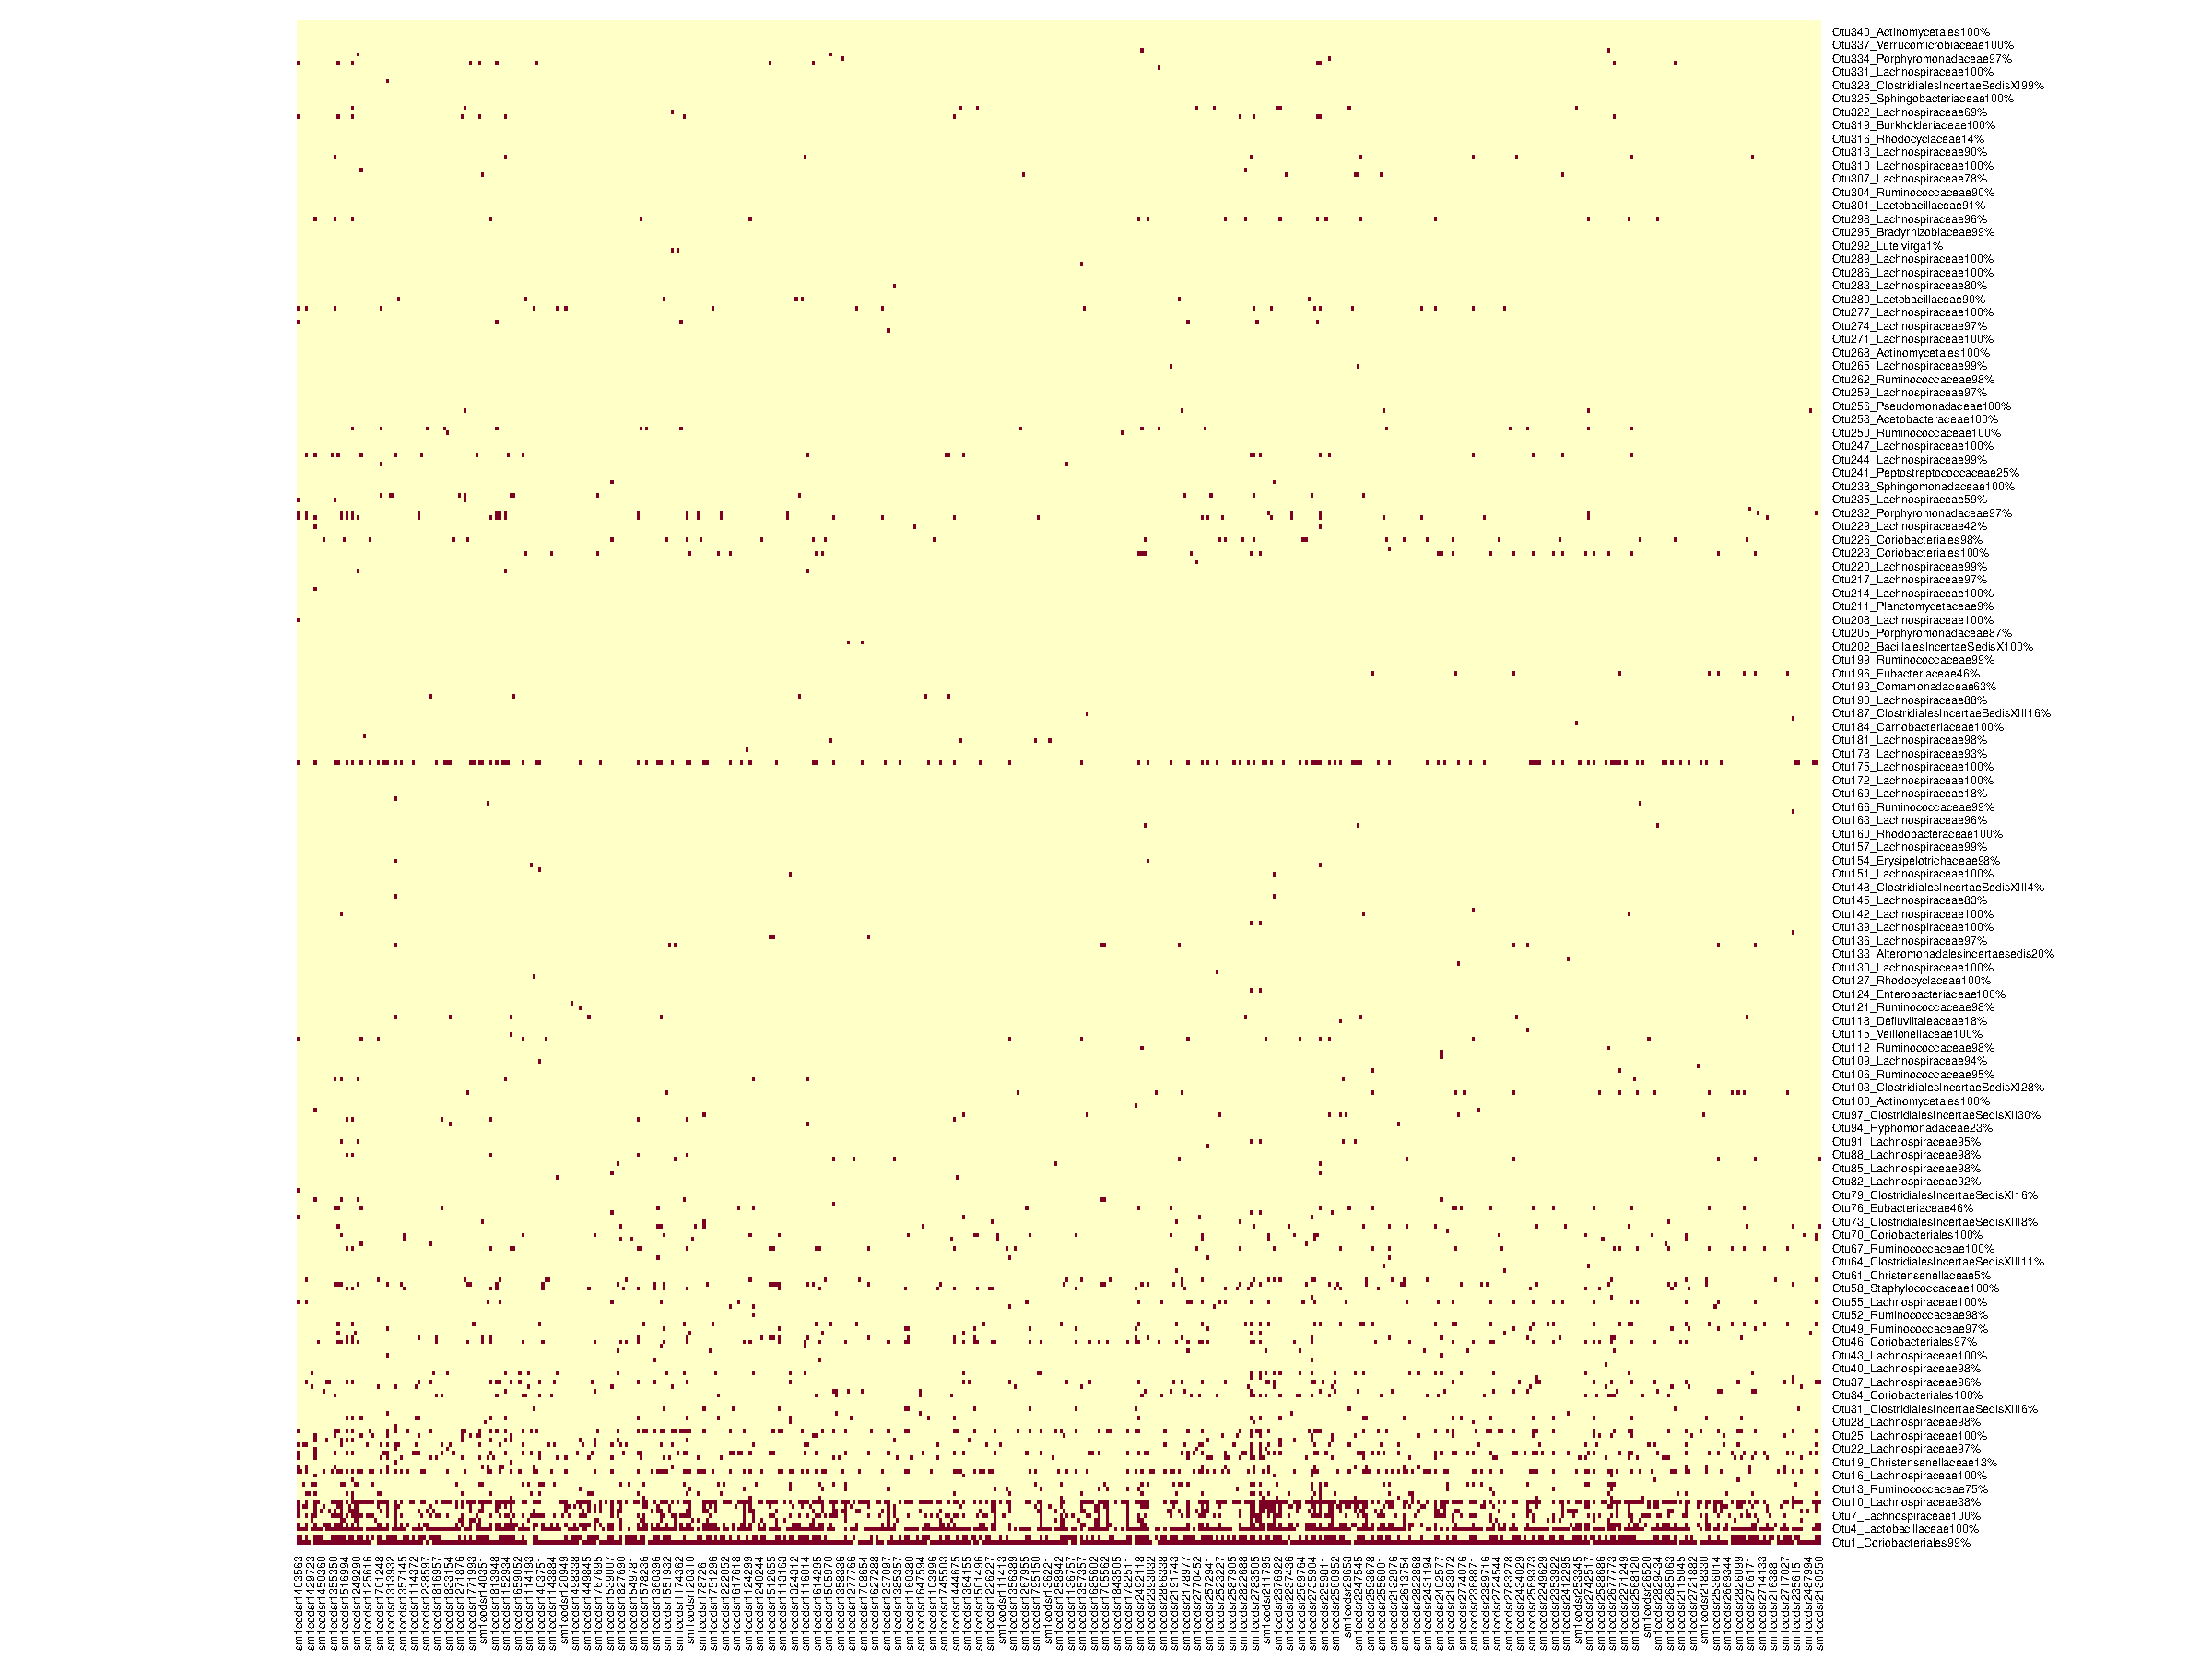
\includegraphics[width=300pt,height=300pt,keepaspectratio]{fig_1_a.pdf}}
	\centerline{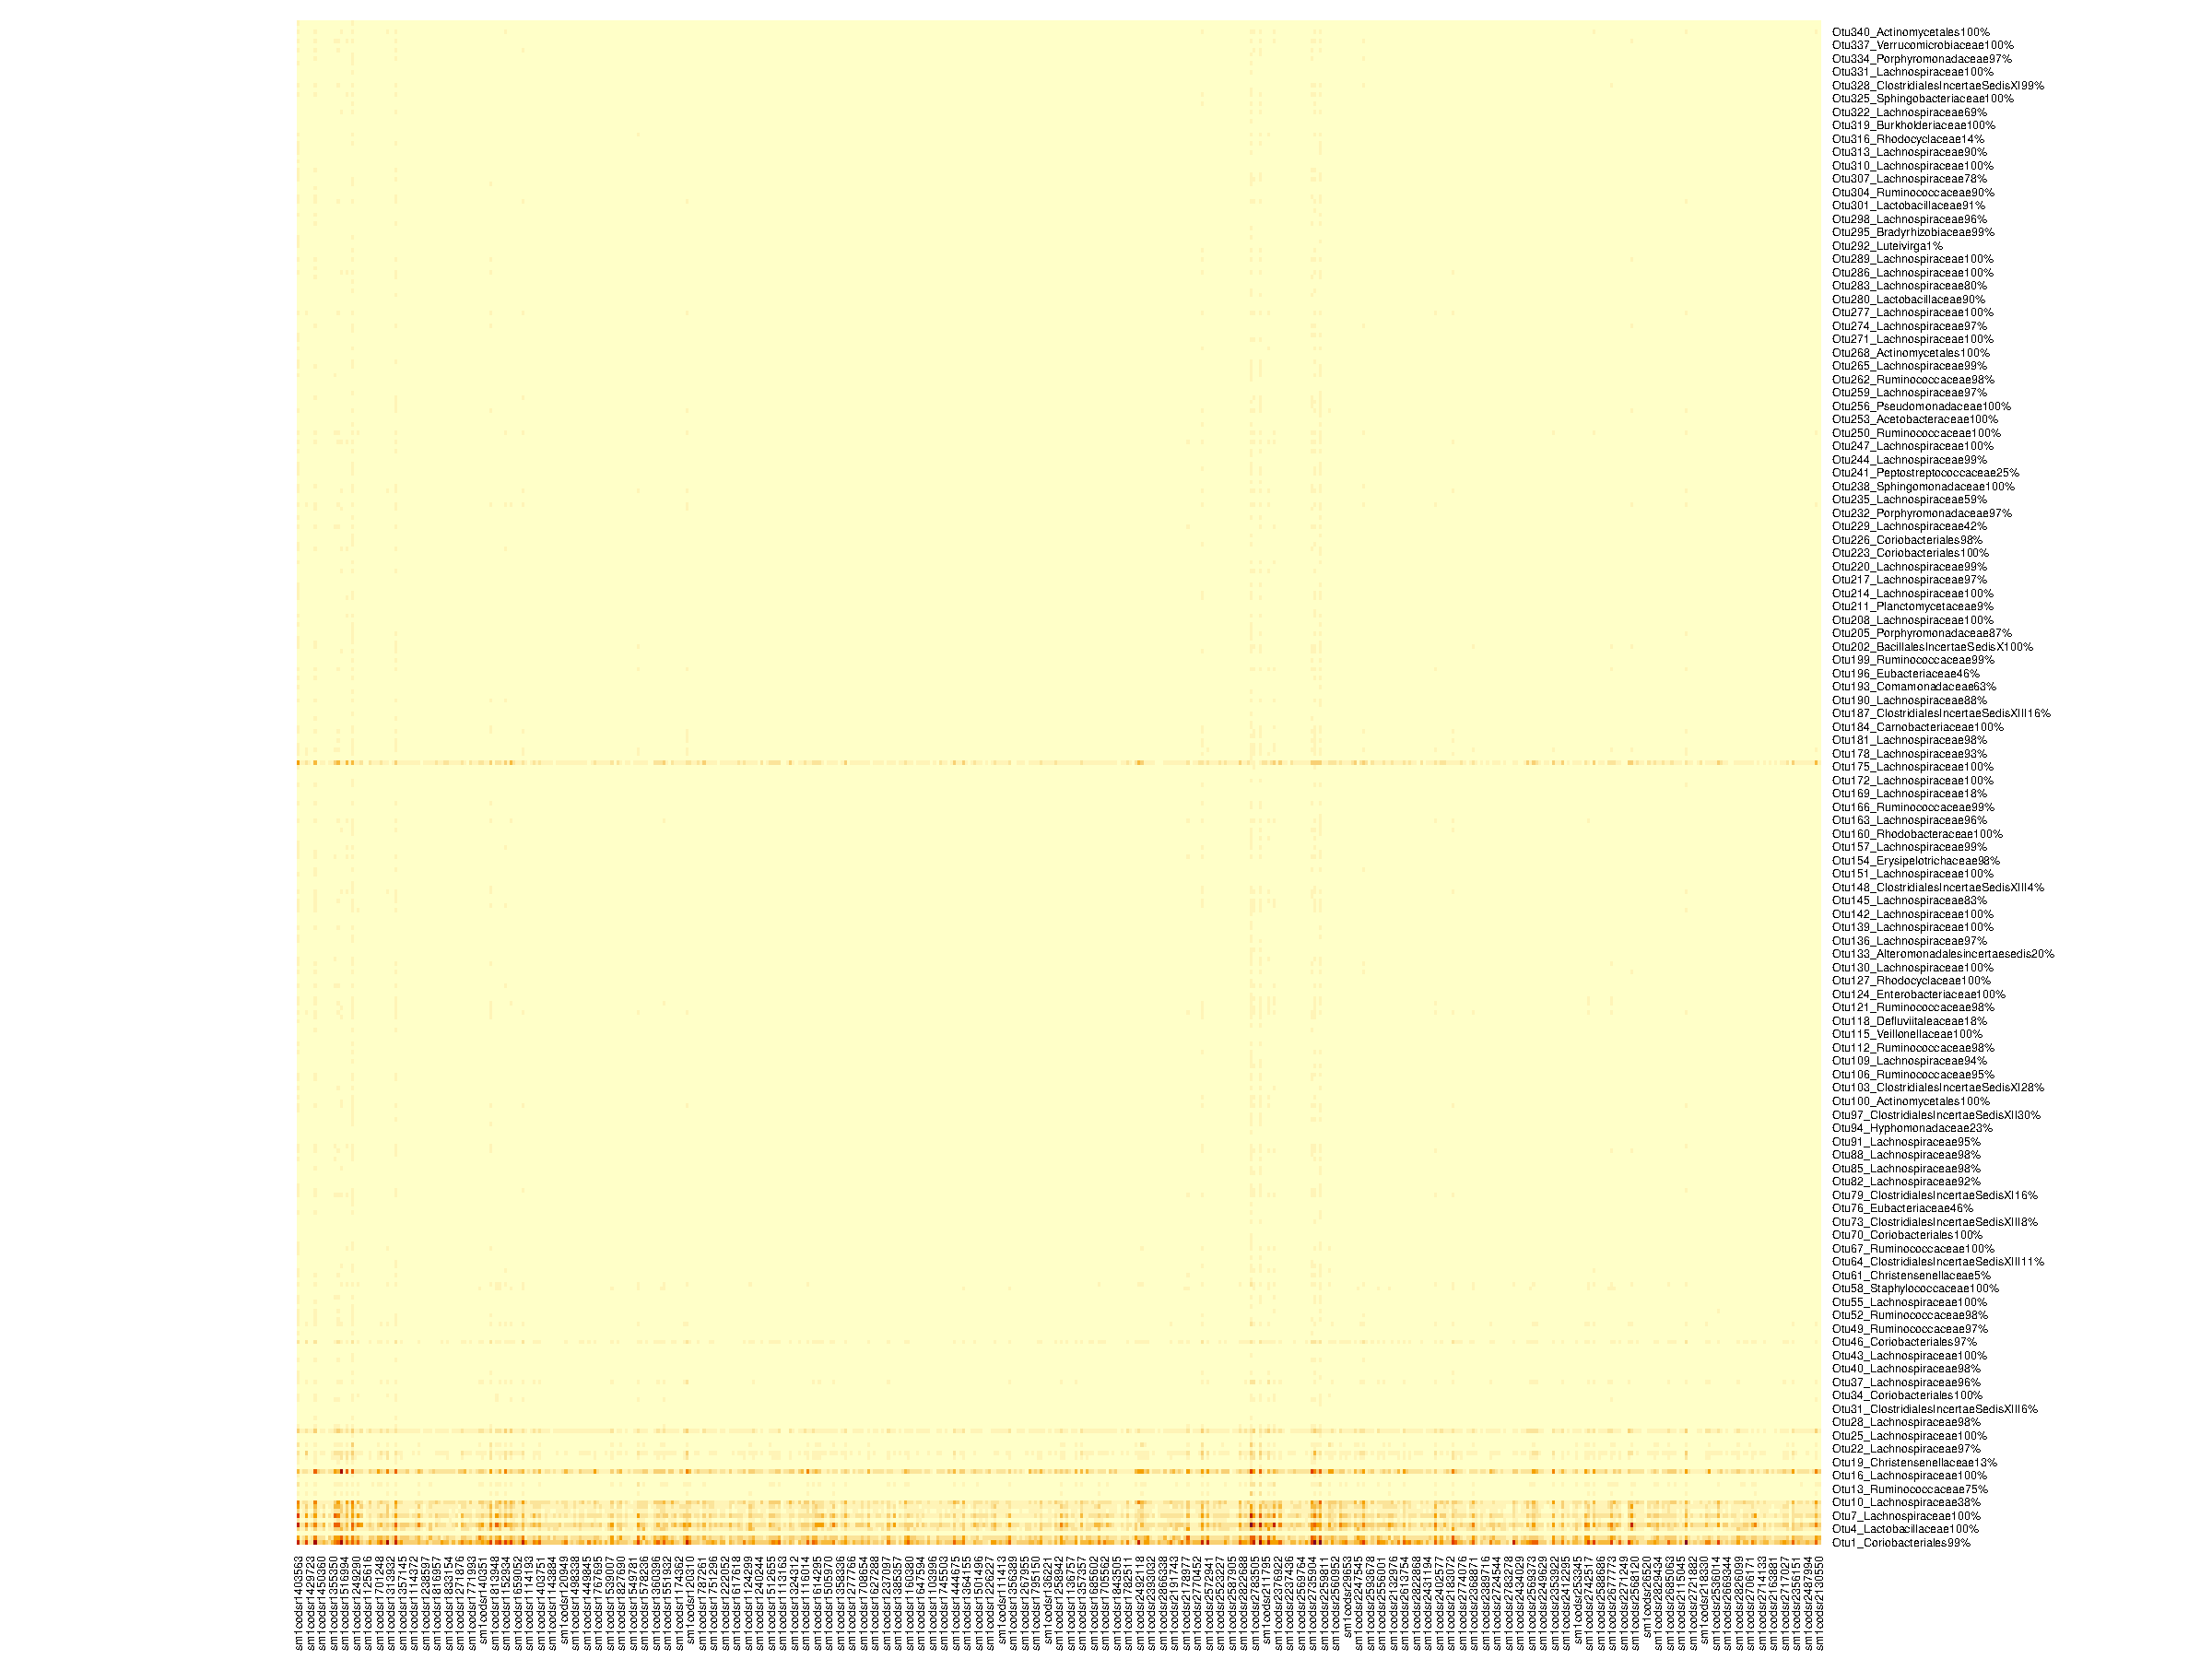
\includegraphics[width=300pt,height=300pt,keepaspectratio]{fig_1_b.pdf}}
	\caption{Top, original profile matrix $\boldsymbol{P}$; bottom, prediction matrix $\boldsymbol{B}\times\boldsymbol{C}$.
	correlation = 0.552, p-value = 0 (Pearson's correlation test)}\label{fig:01}
\end{figure}

\subsection{Functional interpretation of predicted communities}
After successfully predicting community clusters on an OTU level, we next explored whether the bacteria taxa in the same community shared meaningful functional pathways. We applied PICRUSt on top ten mem-bers of each community to obtain functional pathways. (\citealp{Langille2013}).

\subsubsection{Fat metabolism pathways are enriched in communities associated with high fat diet}
Other than the common gut commensal bacteria, we found that bacteria that belong to the phylum \textit{Peptostreptococcae} and \textit{Clostridiaceae} showed distinct enrichment patterns in top communities predicted using MaPS-SEQ data from mice with high fat diet but not in top communities associated with low fat diet (Figure~2\vphantom{\ref{fig:02}}). This finding corroborates a 2019 study that reported increased relative abundance of OTUs belonging to \textit{Peptostreptococcae} and \textit{Clostridiaceae} in rats treated with HFD (\citealp{Liu2019}). 

Furthermore, the most enriched pathway in these communities, the pentose phosphate pathway (NONOXIPENT-PWY), is also strongly implicated in fat metabolism. (Figure~3\vphantom{\ref{fig:03}}) In this pathway, oxidation of glucose is coupled with NADPH synthesis, which then channels energy to fat synthesis (\citealp{Kruger2003}). Therefore, based on these functional analyses, we are confident that our method is indeed able to predict meaningful local functional communities. 

\begin{figure}[!tpb]%figure2
	\centerline{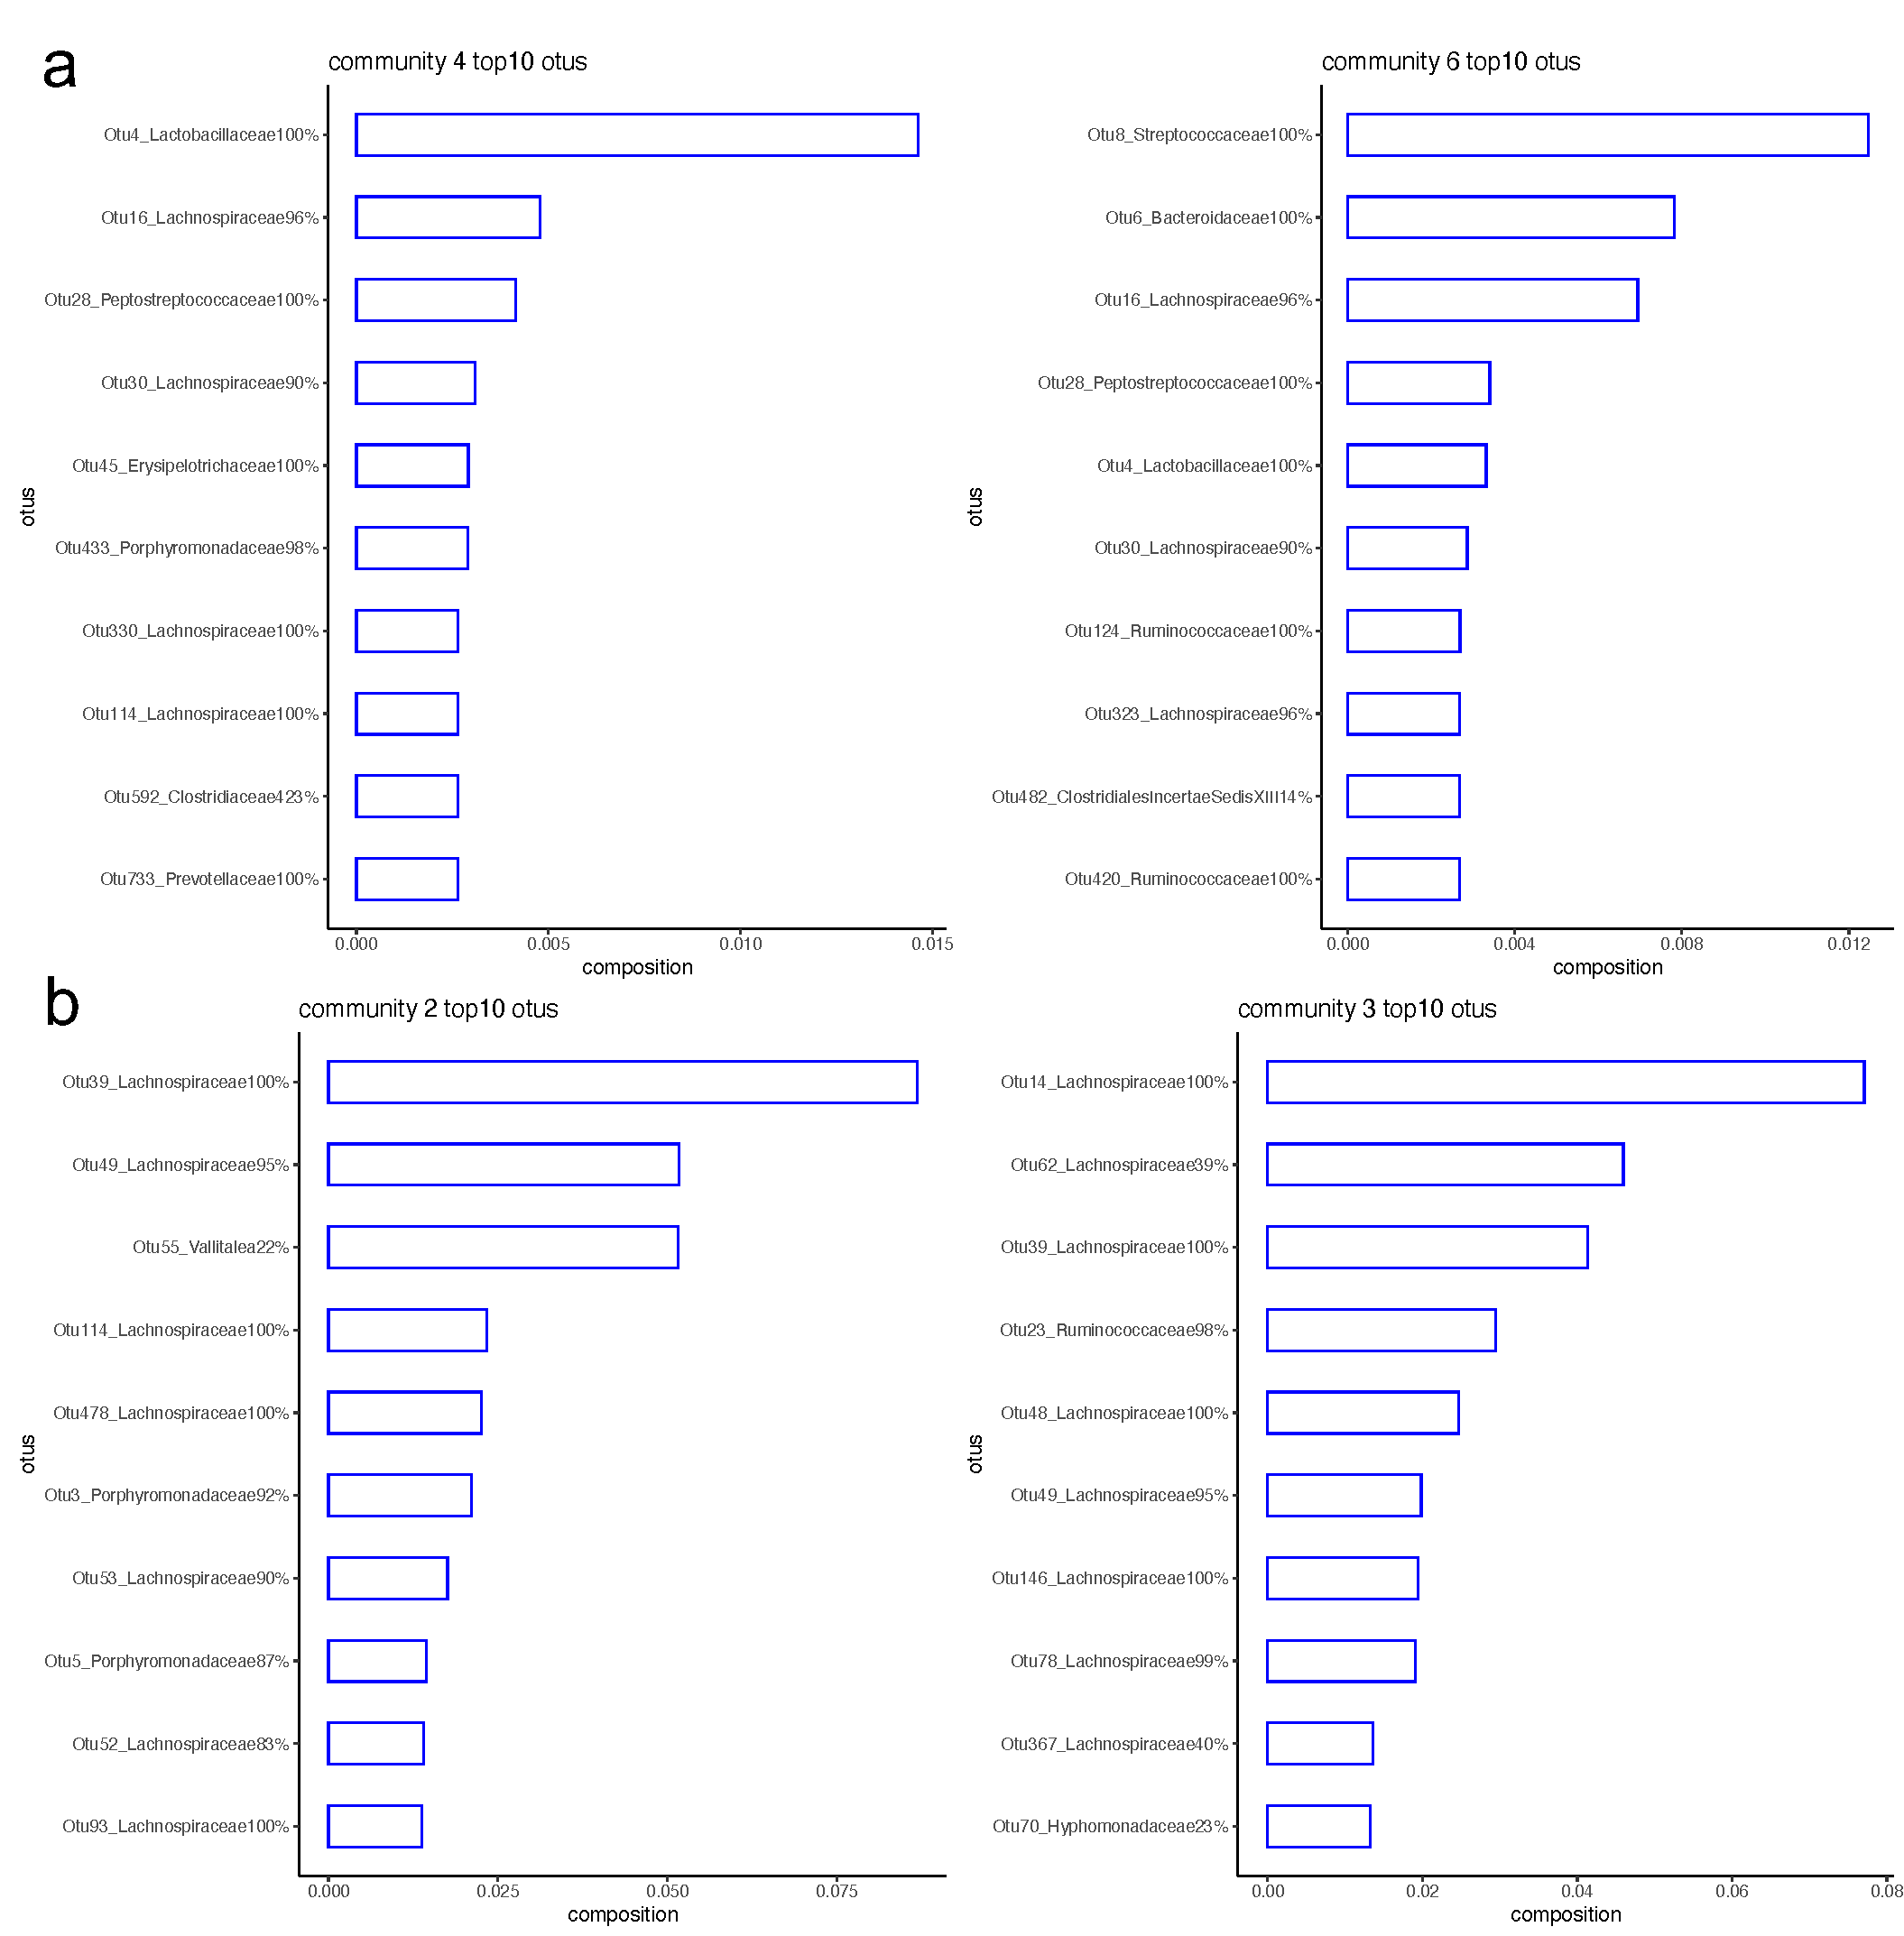
\includegraphics[width=250pt,height=250pt,keepaspectratio]{fig_2.pdf}}
	\caption{2a, left, top10 OTUs of community 4 in the high fat diet mice sample; right, top10 OTUs of community 6 in the same mice sample. 2b, left, top10 OTUs of community 2 in the low fat diet mice sample; right, top10 OTUs of community 3 in the same mice sample. We only show two representative communities in each sample here. X-axis, composition of OTUs in that community. Y-axis, names of top 10 OTUs.} \label{fig:02}
\end{figure}

\subsection{Hierarchical clustering of coefficient matrix}
We observed two different patterns of hierarchical clustering on the coefficient matrix. The samples of high fat mice do not share much coorelations with each other. While in low fat diet mice samples, we observed a gradient-like shape. (Figure~4\vphantom{\ref{fig:04}}) This result indicates that the communities are not evenly distributed among all samples but with a preference to a certain region. Those samples with a higher expression of the communities might spatially locate with each other. The samples with a lower expression in the low fat mice might have communities that cannot be detected by either sequencing technology or this method.


\begin{figure}[!tpb]%figure3
	\centerline{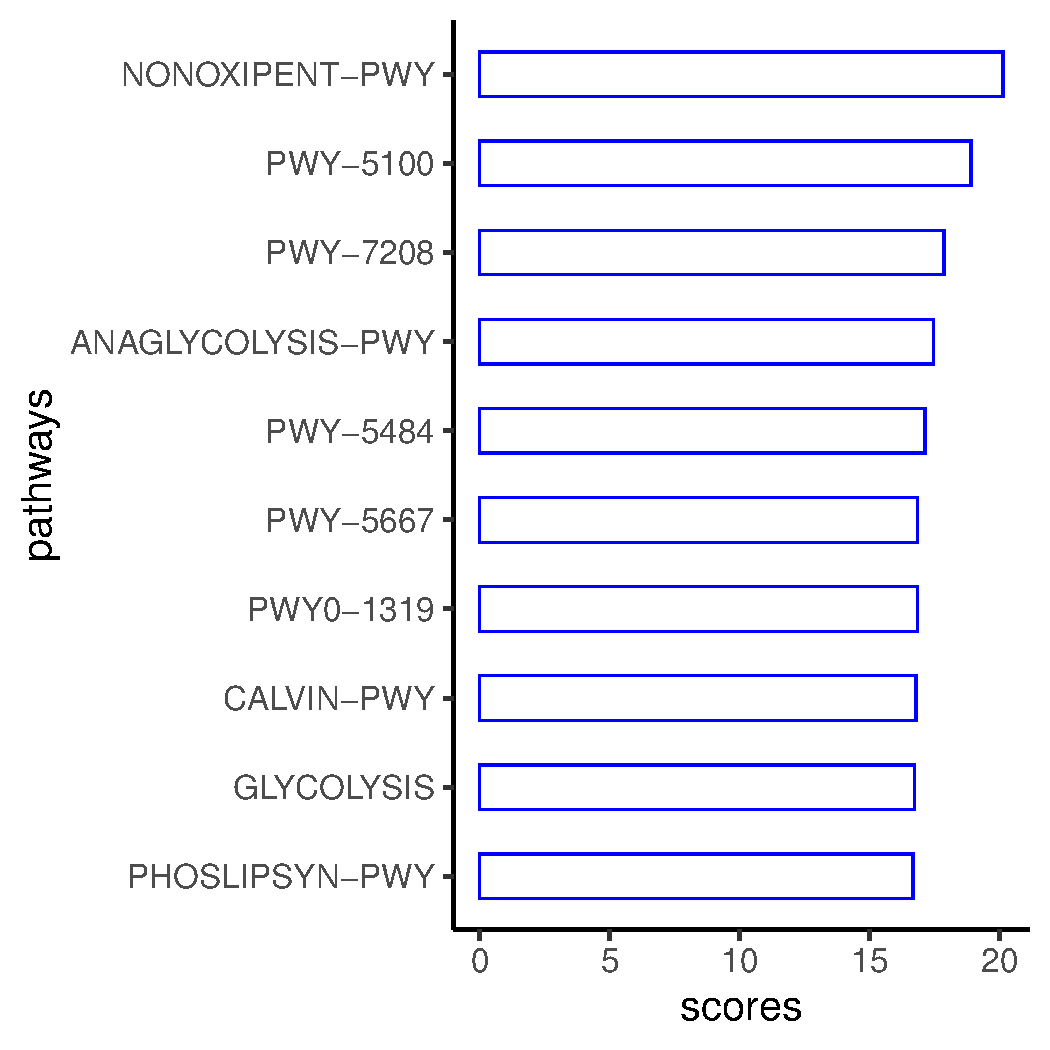
\includegraphics[width=140pt,height=140pt,keepaspectratio]{fig_3_a.pdf}}
	\centerline{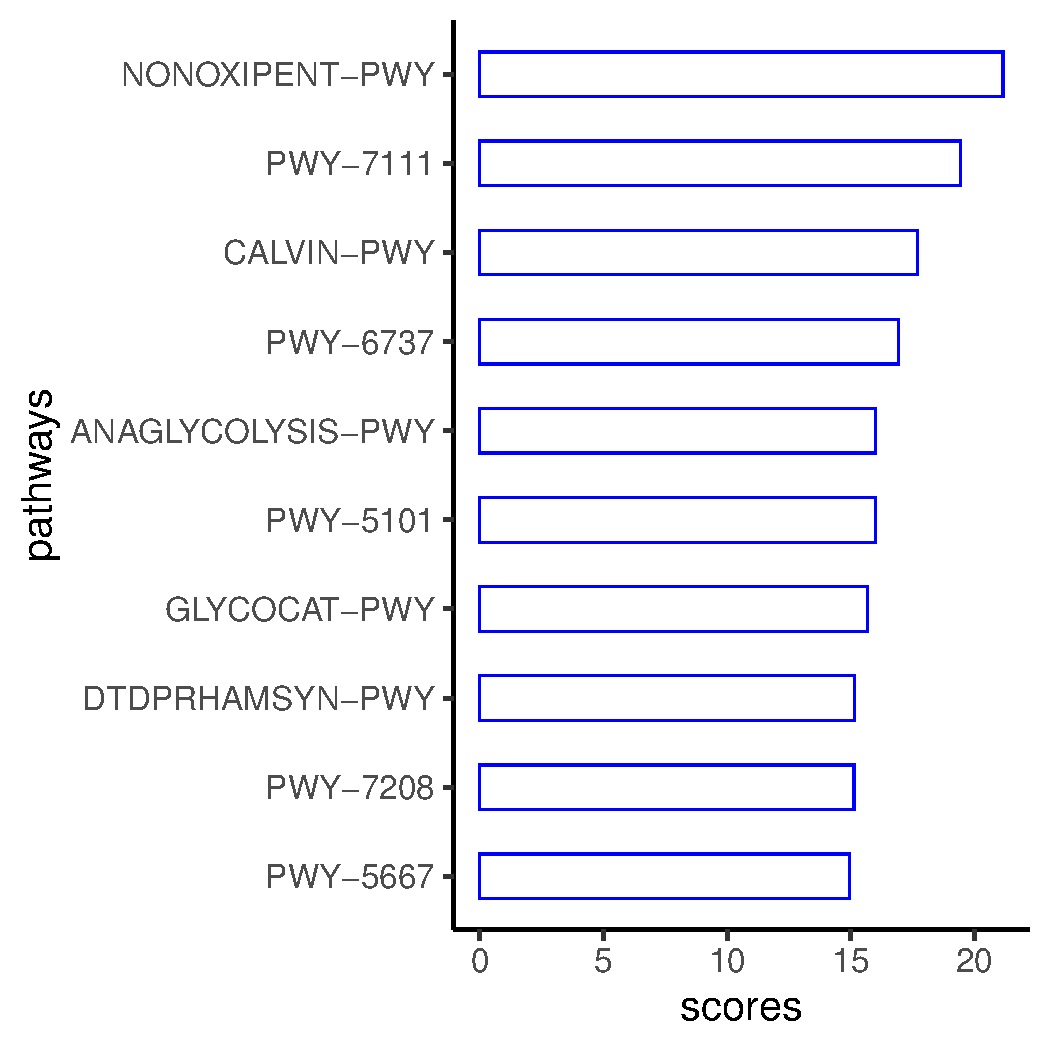
\includegraphics[width=140pt,height=140pt,keepaspectratio]{fig_3_b.pdf}}
	\caption{Top, top10 pathways of community 4 in the high fat diet mice sample. Bottom, top10 pathways of community 6 in the same mice sample; X-axis, enrichment score of pathways predicted by PICRUSt. Y-axis, names of top 10 pathways.}\label{fig:03}
\end{figure}

\begin{figure}[!tpb]%figure4
	\centerline{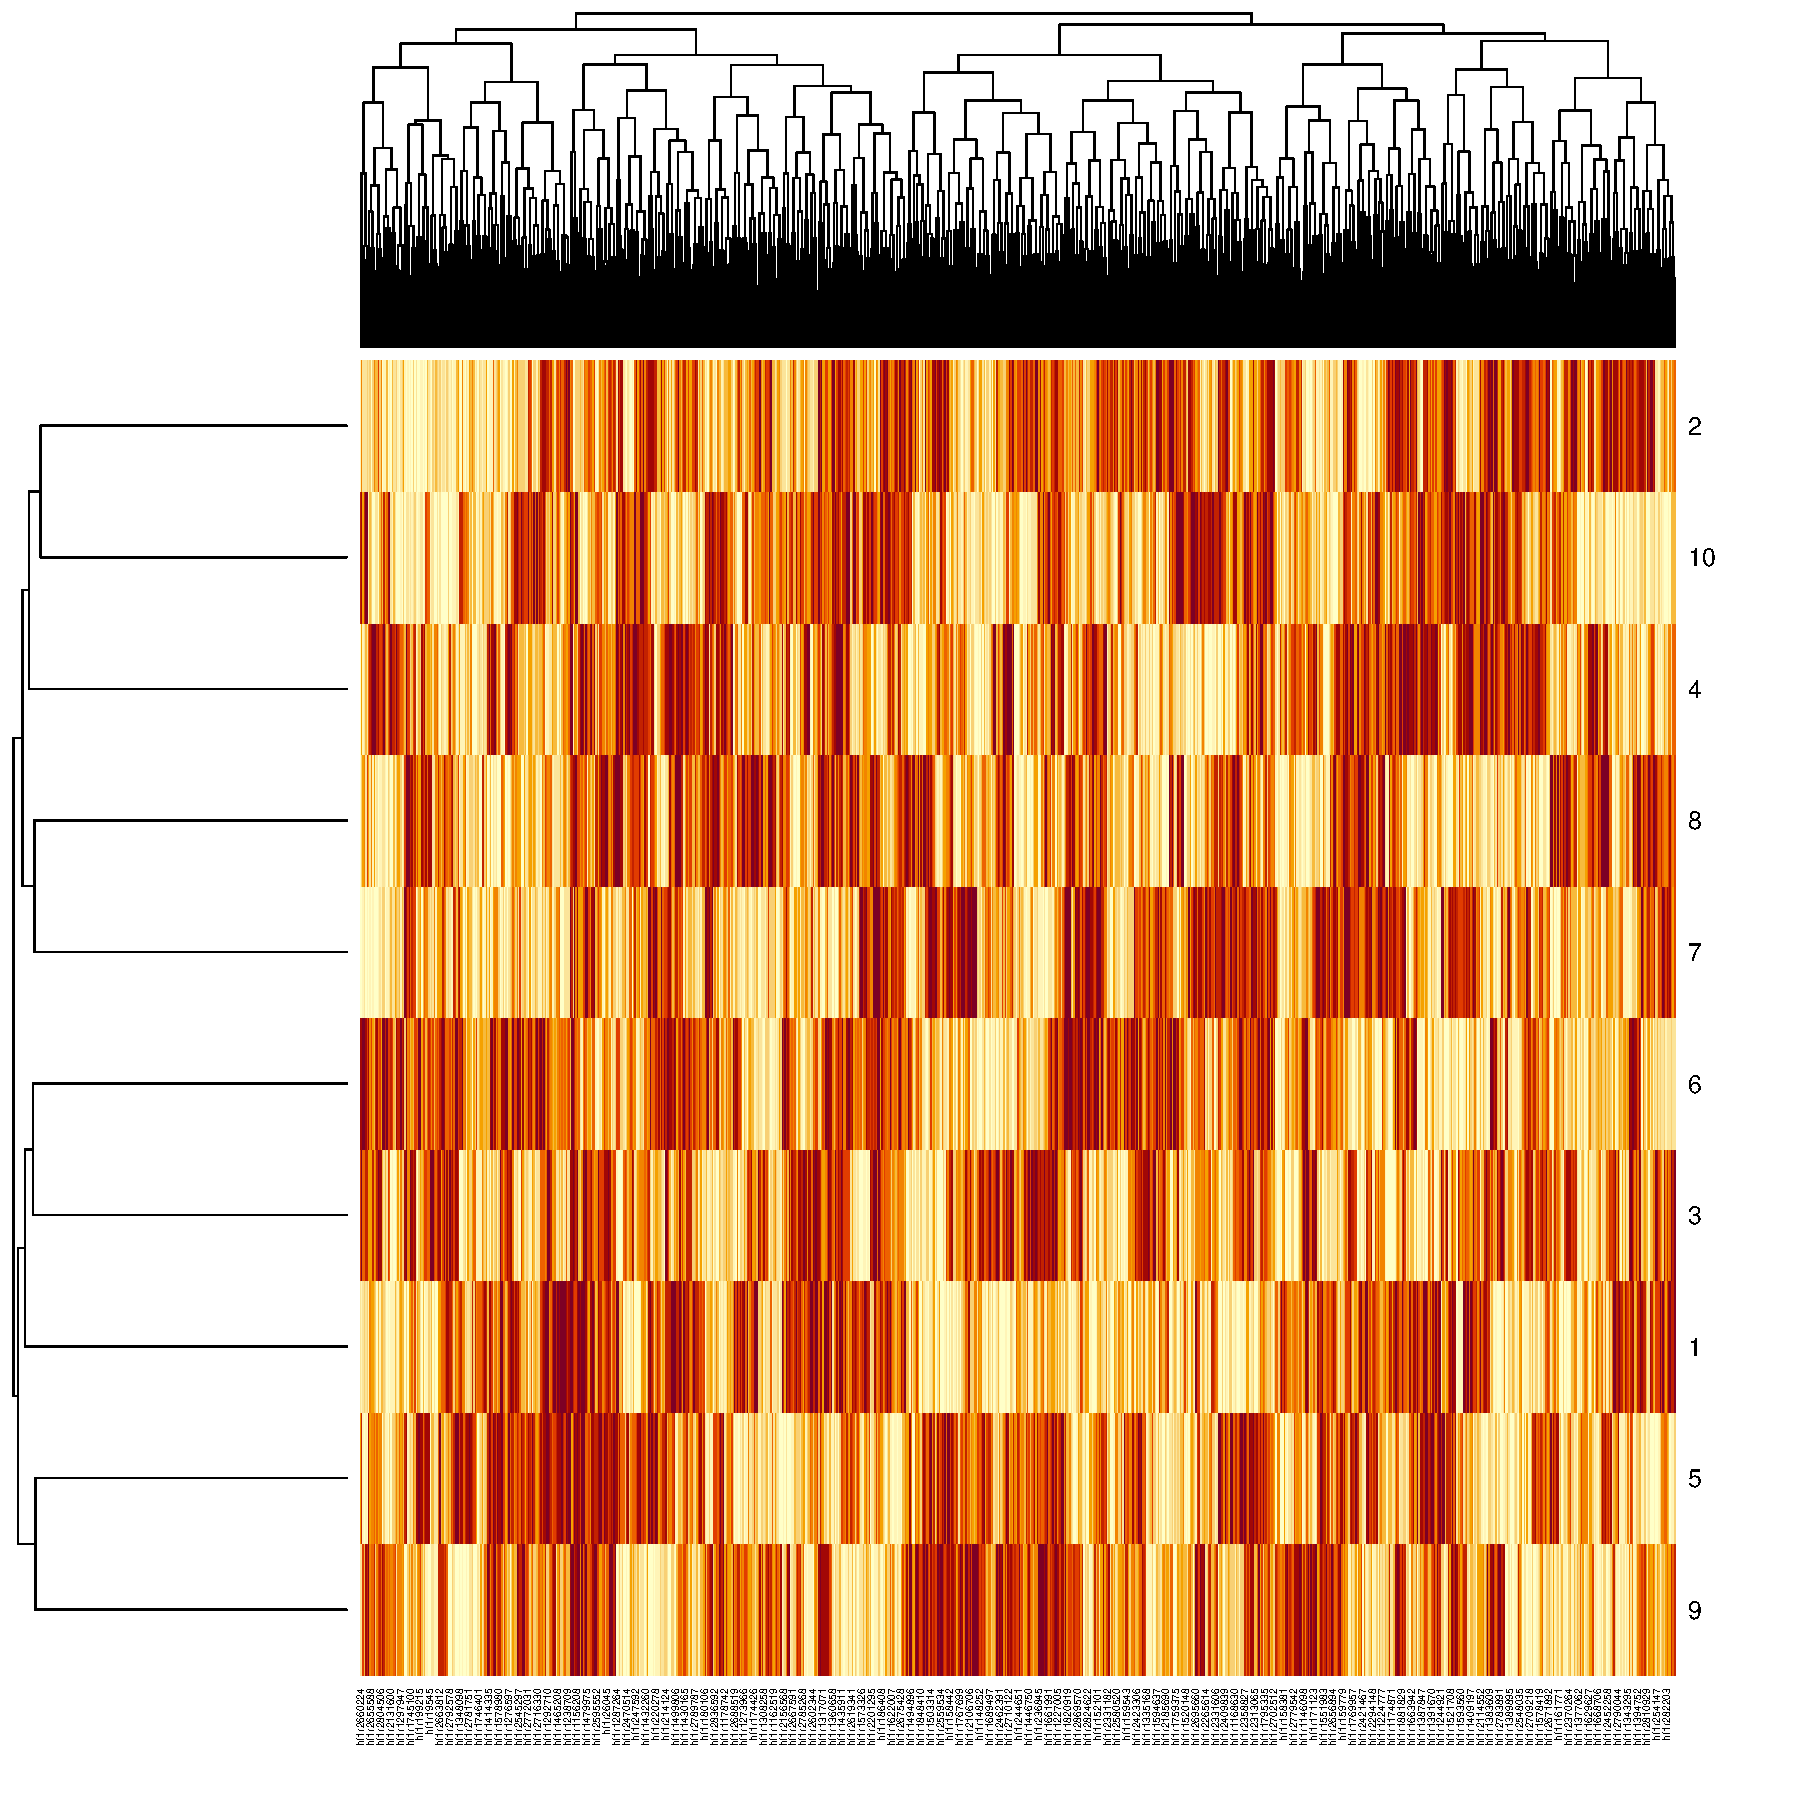
\includegraphics[width=140pt,height=140pt,keepaspectratio]{fig_4_a.pdf}}
	\centerline{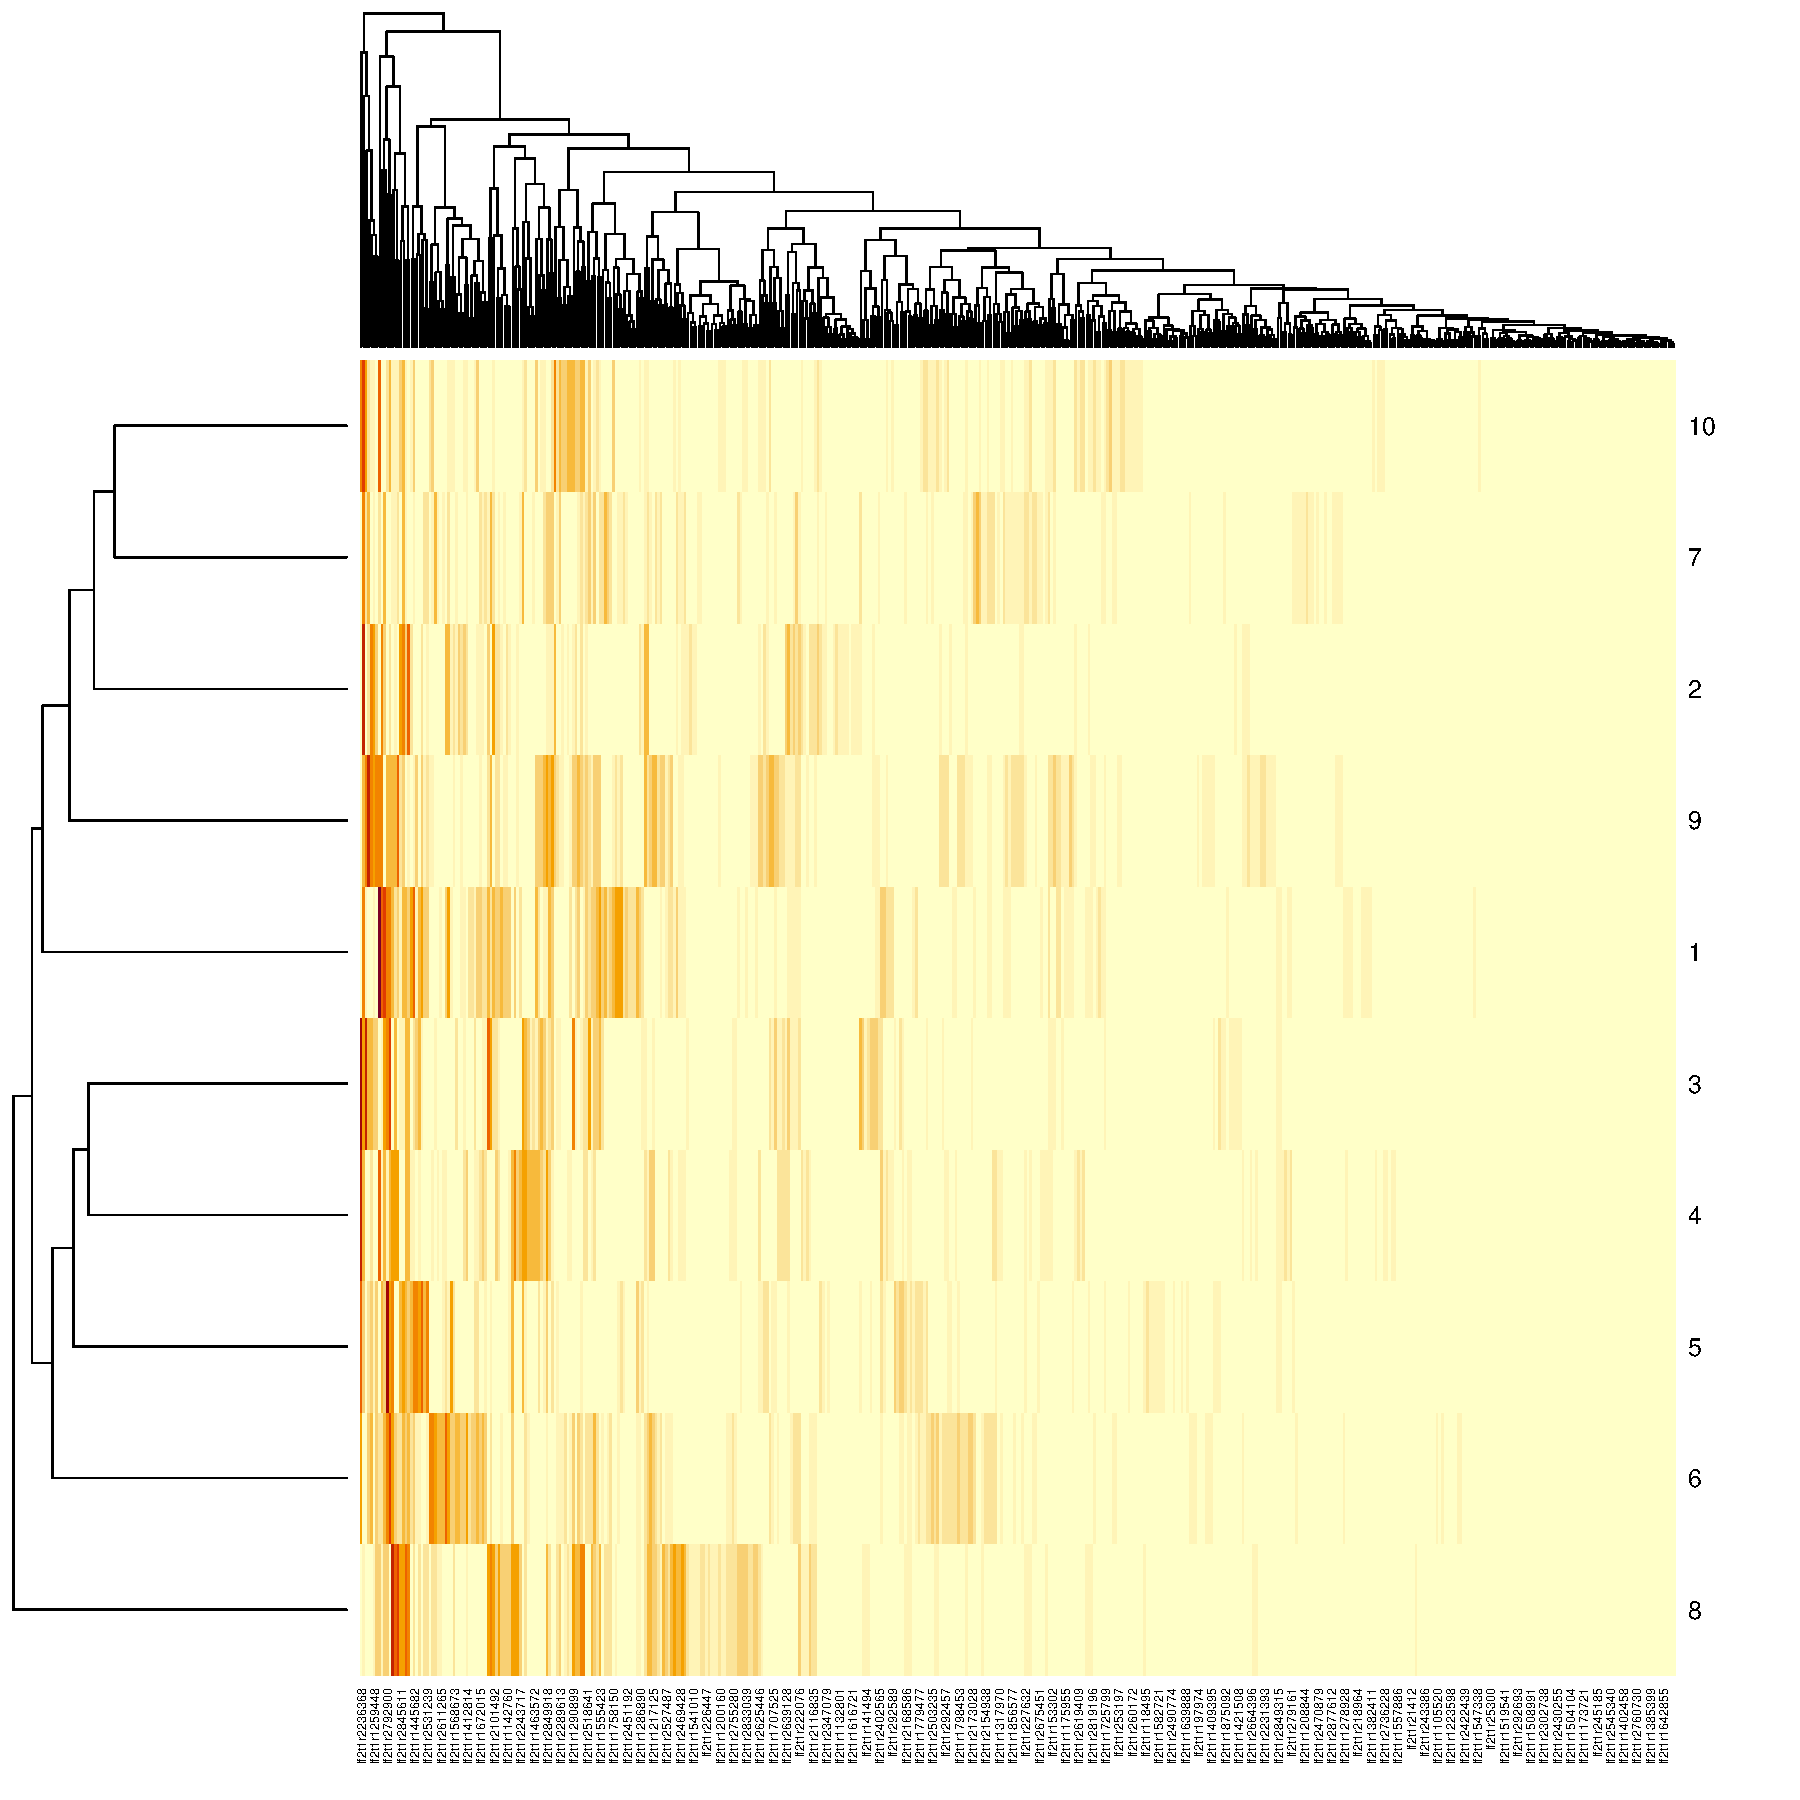
\includegraphics[width=140pt,height=140pt,keepaspectratio]{fig_4_b.pdf}}
	\caption{Top, hierarchical clustering of high fat mice samples; Bottom, hierarchical clustering of low fat mice samples. Columns, samples; Rows, communities.}\label{fig:04}
\end{figure}

\section{Discussion}

In this paper we present a novel computational approach to cluster functional microbiome communities. We used Bernoulli matrix factorization to decompose a sparse operational functional unit (OTU) table from a particular gut compartment and identify potential microbiome communities with local physical interaction and functional cross-feeding. Applying our method to the MaPS-SEQ data, we successfully identified ten putative microbiome communities associated with high-fat diet (HFD). Phylogenetic-based functional pathway analysis further revealed similar metabolic modules related to fat digestion and absorption within each community. Predicted communities associated with different gut regions (ileum, cecum, and colon) share similar profiles. 

However this method has some limitations. First, the optimization is limited by the inital value, we might end up with a local maximum rather than global maximum. Secondly, it is hard to choose the number of latent factors in this model with both good mathematical and biological performance . The third factor that significantly limits our ability to predict local communities lies in the experimental procedure. Due to the PCR amplification errors, the relative abundance counts for each OTU were no longer accurate reflections of their true relative abundance. Therefore, we decided to binarize the counts in our method to reduce confounding biases. To mitigate the PCR issue, we could introduce unique molecular identifiers (UMI) into the particles before PCR, so that UMIs can later be used to demultiplex PCR results.




\begin{thebibliography}{}

\bibitem[Byrd {\it et~al}., 2000]{Byrd2000}
Byrd, R.H., J. C. Gilbert, \& J. Nocedal, (2000) A Trust Region Method Based on Interior Point Techniques for Nonlinear Programming, {\it Mathematical Programming}, {\bf 89}(1), 149-185.

\bibitem[Cordero {\it et~al}., 2016]{Cordero2016}
Cordero, O. X., \& Datta, M. S. (2016) Microbial interactions and community assembly at microscales, {\it Current opinion in microbiology}, {\bf 31}, 227-234.

\bibitem[Coyte {\it et~al}., 2015]{Coyte2015}
Coyte, K. Z., Schluter, J., \& Foster, K. R. (2015) The ecology of the microbiome: networks, competition, and stability, {\it Science}, {\bf 350}(6261), 663-666.

\bibitem[Donaldson \it{et~al}., 2016]{Donaldson2016}
Donaldson, G. P., Lee, S. M., \& Mazmanian, S. K. (2016) Gut biogeography of the bacterial microbiota, \textit{Nature Reviews Microbiology}, \textbf{14}(1), 20-32.

\bibitem[Kruger {\it et~al}., 2003]{Kruger2003}
Kruger, N. J., \& von Schaewen, A. (2003) The oxidative pentose phosphate pathway: structure and organisation, {\it Current opinion in plant biology}, {\bf 6}(3), 236-246.

\bibitem[Langille {\it et~al}., 2013]{Langille2013}
Langille, M. G., Zaneveld, J., Caporaso, J. G., McDonald, D., Knights, D., Reyes, J. A., ... \& Beiko, R. G. (2013) Predictive functional profiling of microbial communities using 16S rRNA marker gene sequences, {\it Nature biotechnology}, {\bf 31}(9), 814.

\bibitem[Lee {\it et~al}., 2013]{Lee2013}
Lee, S. M., Donaldson, G. P., Mikulski, Z., Boyajian, S., Ley, K., \& Mazmani-an, S. K. (2015) Bacterial colonization factors control specificity and stability of the gut microbiota, {\it Nature}, {\bf 501}(7467), 426-429.

\bibitem[Liu {\it et~al}., 2015]{Liu2019}
Liu, H. Y., Walden, T. B., Ahl, D., Nyman, M., Bertilsson, S., Phillipson, M., \& Holm, L. (2019) High‐Fat Diet Enriched with Bilberry Modifies Colonic Mucus Dynamics and Restores Marked Alterations of Gut Microbiome in Rats, {\it Molecular nu-trition \& food research}, {\bf 63}(20), 1900117.

\bibitem[Murtagh {\it et~al}., 1985]{Murtagh1985}
Murtagh F. (1985) Multidimensional Clustering Algorithms, COMPSTAT Lectures 4.


\bibitem[Nagara {\it et~al}., 2017]{Nagara2017}
Nagara, Y., Takada, T., Nagata, Y., Kado, S., \& Kushiro, A. (2017). Microscale spatial analysis provides evidence for adhesive monopolization of dietary nutrients by specific intestinal bacteria, {\it PloS one}, {\bf 12}(4).

\bibitem[Sheth {\it et~al}., 2019]{Sheth2019}
Sheth, R. U., Li, M., Jiang, W., Sims, P. A., Leong, K. W., \& Wang, H. H. (2019). Spatial metagenomic characterization of microbial biogeography in the gut, {\it Nature biotechnology}, {\bf 37}(8), 877-883.

\bibitem[Swidsinski {\it et~al}., 2008]{Swidsinski2008}
Swidsinski, A., Loening–Baucke, V., Verstraelen, H., Osowska, S., \& Doerffel, Y. (2008). Biostructure of fecal microbiota in healthy subjects and patients with chronic idiopathic diarrhea, {\it Gastroenterology}, {\bf 135}(2), 568-579.

\bibitem[Wexler {\it et~al}., 2016]{Wexler2016}
Wexler, A. G., Bao, Y., Whitney, J. C., Bobay, L. M., Xavier, J. B., Schofield, W. B., ... \& Goodlett, D. R. (2016). Human symbionts inject and neutralize antibacterial toxins to persist in the gut, {\it Proceedings of the National Academy of Sciences}, {\bf 113}(13), 3639-3644.


\end{thebibliography}

\end{document}
